\documentclass[lettersize, noapacite, twoside, HRI]{apa_HRI}


%\usepackage[utf8x]{inputenc}
\usepackage{times}

\usepackage{graphicx} 
\usepackage{subfigure}
\usepackage{paralist}

\usepackage{hyperref}

\usepackage{amsfonts}
\usepackage{mathtools}
\usepackage{url}
\usepackage{xspace}
\usepackage{booktabs}

\usepackage[natbibapa]{apacite}


\usepackage{tikz}
\usetikzlibrary{calc,decorations.pathreplacing}
\newcommand{\tikzmark}[1]{\tikz[overlay,remember picture] \node (#1) {};}

\usepackage[draft,nomargin,footnote]{fixme}

\graphicspath{{figs/}}

\newcommand{\eg}{\textit{e.g.}\xspace}
\newcommand{\etal}{\textit{et al.}\xspace}
\newcommand{\ie}{\textit{i.e.}\xspace}
\newcommand{\etc}{\textit{etc.}\xspace}
\newcommand{\vs}{\textit{vs.}\xspace}

\newcommand{\h}[1]{\textbf{H#1}\xspace}

\newcommand{\anti}{{$\mathcal{A}_0$\xspace}}
\newcommand{\antf}{{$\mathcal{A}_1$\xspace}}
\newcommand{\deltaant}{{ $\Delta_{\mathcal{A}_0,\mathcal{A}_1}$\xspace}}


\rightheader{Cognitive Context: Impact on the Perception of a Robot}   % This should be the title, or a shortened version of the title if your title is long.
\leftheader{Lemaignan et al.}	  % For one or two authors, include both authors last names.  For three or more, use first author's last name et al.
\title{Cognitive Context: Impact on the Perception of a Robot}

\author{S\'everin Lemaignan, Kshitij Sharma, Ashish Ranjan Jha, Pierre
Dillenbourg}
\affiliation{CHILI Lab, \'Ecole Polytechnique F\'ed\'erale de Lausanne}

\acknowledgements{\url{firstname.lastname@epfl.ch}}

\abstract{
What leads us to attribute human-like characteristics to robots? The physical
appearance of the robot and the design of its behaviours do obviously play a key
role. This paper however reveals another mechanism at play, which is more subtle
and partially unconscious: the context of the interaction, and more precisely,
the cognitive prerequisites that the interaction presupposes.

To study this effect, we propose an original methodology based on eye-tracking
and a set of stimuli that are visually identical and yet induce different
assumptions regarding the cognitive capabilities of the robot. We then correlate
the gaze patterns with established questionnaires that assess anthropomorphic
attributions.

\begin{inparaenum}[\itshape a\upshape)]
As a result, we show that \item specific gaze patterns (fixations on the head of
the robot) correlate with post-hoc anthropomorphic
attributions, and hence, eye-tracking can be used as a novel \emph{in-the-moment}
metric of anthropomorphism, and \item simple context priming is sufficient
to elicit significantly different anthropomorphic attributions.
\end{inparaenum}

}

\keywords{human-robot interaction, anthropomorphism, cognitive context, eye-tracking, gaze patterns}

\begin{document}
\maketitle

\section{Introduction}

Robotics researchers often tend to consider that anthropomorphism only describes
a static set of human-like features of a robot (like its shape, its speech
capabilities, facial expressions, etc.).
Following~\citet{fink_anthropomorphism_2012}, we refer to these characteristics
as the \emph{anthropomorphic design} of the robot, and we call
\emph{anthropomorphism} the general \emph{social phenomenon} that emerges from
the (real or imagined) interaction between a non-human agent (a robot in our
case) and a human~\citep{persson_anthropomorphism_2000}.  According
to~\citet{epley_when_2008}, anthropomorphism includes the human perception of
emotional states, motivations, intentions in the non-human agent, and tends to
ascribe those qualities to it. As such, the dynamic and socio-cognitive
dimensions of anthropomorphism are essential to understand the complex bonds
that human users build with artificial agents such as
robots~\citep{lemaignan2014dynamics}. Therefore we propose therefore that
anthropomorphism can be a useful \emph{proxy} to these intricate psychological
bonds. This article aims at improving our understanding of this phenomenon
\textbf{by evidencing the impact of the cognitive presuppositions implied by the
context of the interaction}.

The study of context in HRI is not new. \textit{Context of use} is defined by
the ISO as \textit{``users, tasks, equipment (hardware, software and materials),
and the physical and social environments in which a product is used''}.
Accordingly, there are various aspects that can impact how a robot is
experienced. The real or imagined \textit{purpose} of a robot, including the
application context in which it is typically used (\eg office environment, home,
rehabilitation center, public space, \etc) as well as the task context (\eg
serious or playful task; composition of human-robot team; number of users) and
the (social) role in which the robot is used / experienced are taken into
account. Generally, when the context of use of a robot is social, entertaining
or playful, it will enhance anthropomorphism compared to when the context is a
routine or focused serious task (security, rescue, \etc).
\citet{joosse_what_2013} showed, for instance, that when the same robot ({\sc
nao}) was used in a different task context (cleaning task \vs tour guide), users
ascribed different personalities to the robot. \citet{goetz_cooperation_2002}
revealed a link between a robot's context of use and people's perception of the
robot: the authors found that people prefer a serious robot for serious tasks
and a less serious robot for more playful tasks. \citet{kaplan_free_2000}
discussed the role of uselessness in the design of robots. The author argues
that artificial pets like AIBO have no real purpose, in a sense that they do not
provide any kind of service or, in other words, \textit{``they are not doing
what you tell them to do''} and \textit{``they might refuse the order of its
owner''}. It may be this very aspect that increases people's tendency to
anthropomorphize the robot. According to Kaplan, it is in our daily use language
that we tend to attribute intentions to devices that are not doing their job
well.

These previous studies investigated users' perception of robots in
prototypical situations (routine \vs playful, typically boring \vs typically
intellectual) and their results nicely supports our general intuition.
In this article, we show that much more subtle variations in the task context do
lead to very noticeable effects as well.

\subsection*{Measuring anthropomorphism}

Measuring anthropomorphism raises
interesting methodological challenges, if only because people's perception of
robots change over the duration of their interaction with the
robots~\citep{lemaignan2014dynamics}. \citet{takayama_perspectives_2012}
discusses the effects of these changes and differentiates between what she calls
an \emph{in-the-moment} and a \emph{reflective} perspective on agency: an
\emph{in-the-moment} perspective would refer to one's most immediate
response/sense in a given situation whereas a \emph{reflective} perspective would
indicate one's reaction/sense of a situation based on a more in-depth
consideration and contemplation.  In the first phase of interaction with a
robot, people might respond ``mindlessly'' instead of responding
consciously~\citep{nass_machines_2000}, and only after what is called the
\emph{familiarization} period, one might respond in a more reflective manner
instead of an in-the-moment reaction: \citet{reeves_media_1996} showed for
instance that subjects interacting with technologies in ways close to how they
would behave towards people, would deny any human-like interaction in a post-hoc
questionnaire, illustrating this reflective perspective.

Yet, most of the experiments that investigate anthropomorphism in HRI are based
on post-interaction, closed questionnaires or rating scales.  The Godspeed
questionnaire~\citep{bartneck_measurement_2008}, and in particular, its subpart
focused on anthropomorphism, is the main validated questionnaire to assess
anthropomorphism. On 5-points semantic differential scales, people are asked to
rate the following constructs: fake \vs natural, machinelike \vs humanlike,
unconscious \vs conscious, artificial \vs lifelike, moving rigidly \vs moving
elegantly. Because the concept of ``human-likeness'' itself is complex and
abstract, \citet{kahn_jr._robotic_2006} suggest to ask for more concrete
constructs that are typical or unique of the concept of ``human-likeness'', and
\citet{ruijten_introducing_2014} propose for instance a 25-item questionnaire to
measure various concrete aspects of human-likeness. Other
researchers~\citep{zlotowski2014dimensions,salem2015would} also applied a
two-dimensional scale measuring \emph{Human Nature} and \emph{Uniquely Human}
traits of robots, based on an original proposal by \citet{haslam2008attributing}.

We take here a different approach to measure anthropomorphism, based on
eye-tracking.  By looking at the eyes fixation on the head of the robot, we have
been able to demonstrate significantly different patterns in two experimental
conditions subtly different in terms of human-likeness. This eye-tracking based
metric is behavioural and hence does not suffer post-hoc reconstruction by the
subjects, possibly providing a better, ``noise-less'', access to the human
attitude towards the machine, and, as such, a better proxy to the cognitive and
affective bonds that the human establishes with the robot.


\subsection*{Hypotheses}

The study has been designed out of the following intuition: \emph{the more we
ascribe cognitive capabilities to an agent, the more we focus on its head when
interacting with it}.  Eye-tracking was a natural methodology to investigate
this intuition, and we crafted audio-visual stimuli that would elicit different
levels of cognitive ascription onto the robot while being identical in every
other way.

Several hypotheses ensued, our baseline hypothesis \h{0} being that \emph{shallow
cognitive contexts} and \emph{deep cognitive contexts} are recognized
(manipulation check) and interpreted by the participants as being respectively
\emph{machine-like} (low level of anthropomorphic attributions) or
\emph{human-like} (higher level of anthropomorphic attributions).

Our first hypothesis \h{1} is that gaze behaviour alone is sufficient to
know if a subject is looking at a robot or at a human.  More precisely, we
hypothesize that the distribution of gaze fixations on the different body parts
is significantly different when watching a robot or a human performing the same
task.

Secondly, we hypothesize (\h{2}) that the \emph{difference} of gaze
behaviours between the human and robot conditions correlates with the
participants' initial tendency to anthropomorphize, measured from a standard
pre-questionnaire: we expect that people with high tendency to anthropomorphize
will tend to have smaller differences in their gaze behaviours while watching
either a robot or a human performing the same task.

Then, we hypothesize (\h{3}) that the gaze fixations on the head are significantly
different depending on the cognitive context, and that a deeper cognitive
context corresponds to longer gaze fixations on the head. This would in turn
interpreted at \emph{gaze fixations on the head is a proxy for an higher
level of human-likeness attribution}, the core hypothesis of this article.

Finally, the hypothesis \h{4} examines whether the cognitive context affects the
general tendency to anthropomorphize, \ie whether observing a
robot acting in an \emph{human-like} context leads to an increased level of
anthropomorphic attributions to robots (and vice versa). This also provides us
with a way to triangulate the behavioural measures with the subjective
attribution of anthropomorphism.

\section{Experimental Design}

As hinted, this study is build as an eye-tracking experiment (using a stationary
eye-tracker SMI RED 250) where participants watch short videos of an agent --
either a robot (Aldebaran Robotics' Nao) or a human -- performing very simple
task (picking an object or pointing toward a sound source), in two different
socio-cognitive contexts.  These contexts, created by priming and/or audio cues,
are designed to elicit either a shallow cognitive context (that participant
would refer as a \emph{machine-like situation}) or a deeper cognitive context
(refered as a \emph{human-like situation}).

Besides eye-tracking, the participants' perception of robots is assessed through a
pre- and a post-questionnaire interaction, described below.

\subsection{Conditions}

The study follows a 2$\times$2 design, summarized in table~\ref{table:design}. Our two
independent variables are the level of socio-cognitive context (\emph{shallow
cognitive context} \vs \emph{deep cognitive context}) and the nature of the
agent appearing in the stimulus (a \emph{robot}, eliciting a \emph{human-robot} interaction
situation, or a \emph{human}, eliciting a \emph{human-human} interaction
situation).

\begin{table}
    \centering
    \small

    \tikzmark{top}

    \tikzmark{left}
    \begin{tabular}{l|p{4cm}|p{4cm}}
        & \tikzmark{top1} Shallow cognitive context & Deep cognitive context \tikzmark{top2}  \\
        \hline
        \tikzmark{left1} Robot & {\bf A}: \emph{``Pick the brown toy''} & {\bf A}: \emph{``Pick your favorite toy''} \\
                               & {\bf B}: \emph{``Point at the noise''} & {\bf B}: \emph{``Point at the crying baby''} \\
        \hline
        \tikzmark{left2} Human & {\bf A}: \emph{``Pick the brown toy''} & {\bf A}: \emph{``Pick your favorite toy''} \\ 
                               & {\bf B}: \emph{``Point at the noise''} & {\bf B}: \emph{``Point at the crying baby''}\tikzmark{bottom} \\
        \end{tabular}

    % draw the over- and side-braces
    \begin{tikzpicture}[overlay, remember picture]

        \draw [decoration={brace,amplitude=0.5em},decorate,thick]
        (top -| top1.west) --  (top -| bottom.east) node[midway, above=0.5em] {\scriptsize between subjects};

        \draw [decoration={brace,amplitude=0.5em},decorate,thick]
        ($(left |- bottom)+(1.8,-0.3)$) --  ($(left |- left1.north)+(1.8,0.2)$) node[midway,above=3em,left=1em,rotate=90] {\scriptsize within subject};
    \end{tikzpicture}
    %%%

    \caption{\small The study follows a 2$\times$2 design: the \emph{robot} vs
        \emph{human} condition is within subject, while the \emph{shallow
        cognitive context} \vs \emph{deep cognitive context} is between subject.
        Two stimuli (\emph{Picking} task, {\bf A}, and \emph{Sound} task,
        {\bf B}) were shown to the participants, introduced by brief verbal
        commands, reproduced in the table. Figure~\ref{fig:stimuli} shows
        pictures of the four stimuli.}

    \label{table:design}
\end{table}


\subsection{Video Stimuli}

Four different video stimuli where filmed (figure~\ref{fig:stimuli}): two
different tasks (picking a stuffed animal, refered hereafter as the
\emph{Picking} task, and pointing towards a source of sound, refered as the
\emph{Sound} task) acted either by a human or a robot. Video stimuli were
realised in studio conditions. All videos followed the same simple structure: an
initial audio command (spoken by an invisible person), followed by the task
being executed.

The human actor was instructed to follow as closely as possible the actions and
attitudes of the robot (left/right glances, hesitations\ldots), while keeping a
natural, \emph{human-like} general behaviour.  Hence, the length of human videos
(57 seconds in total for the two tasks) was shorter than robot videos (110
seconds) due to the robot being usually slower in performing actions (in
particular walks) compared to human.

The audio (and audio only) of these four videos was then edited to create two
sets of stimuli: one for the \emph{shallow cognitive context} condition, one for
the \emph{deep cognitive context} condition. The audio editing consisted in
inserting different commands to initiate the tasks (reported in
table~\ref{table:design}): in the \emph{Picking} task for instance, the object
that the agent had to pick was described either as a \emph{``brown toy''} or as
\emph{``your favorite toy''}. In the former case, the object was refered through
visible, objective features which do not suppose as deep cognitive capabilities
as in the latter case where the agent is implicitly supposed to have
tastes and preferences such as it can choose a toy as its favorite.

This simple verbal priming (\emph{``brown toy''} \vs \emph{``your favorite
toy''}) set the cognitive context (\emph{shallow} \vs \emph{deep}) and was
expected to lead to different perceptions of the interaction
(\emph{machine-like} \vs \emph{human-like}). We reinforced this effect in the
\emph{Sound} task: not only the verbal priming but also the sound played by the
speakers during the task was altered: either a repetitive bip (\emph{shallow
cognitive context}) or the sound of a crying baby (\emph{deeper cognitive
context}).

\begin{figure}
    \centering
    \subfigure[\emph{Picking} task, robot condition]{
        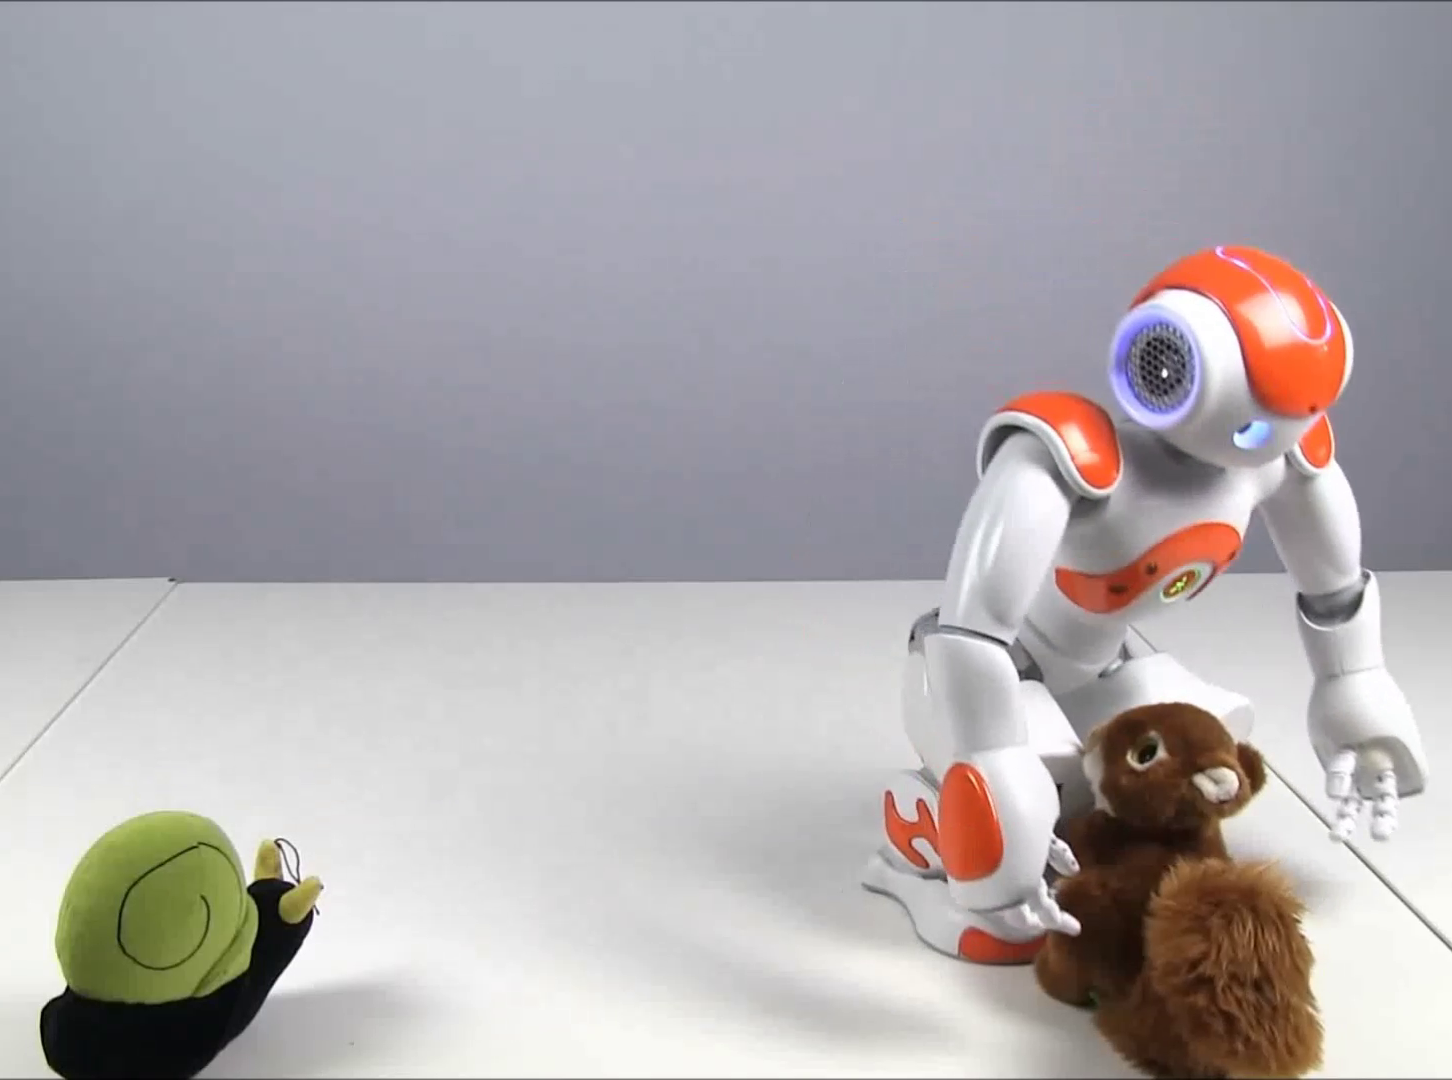
\includegraphics[height=5cm]{stimulus-robot-toys}
    }
    \subfigure[\emph{Picking} task, human condition]{
        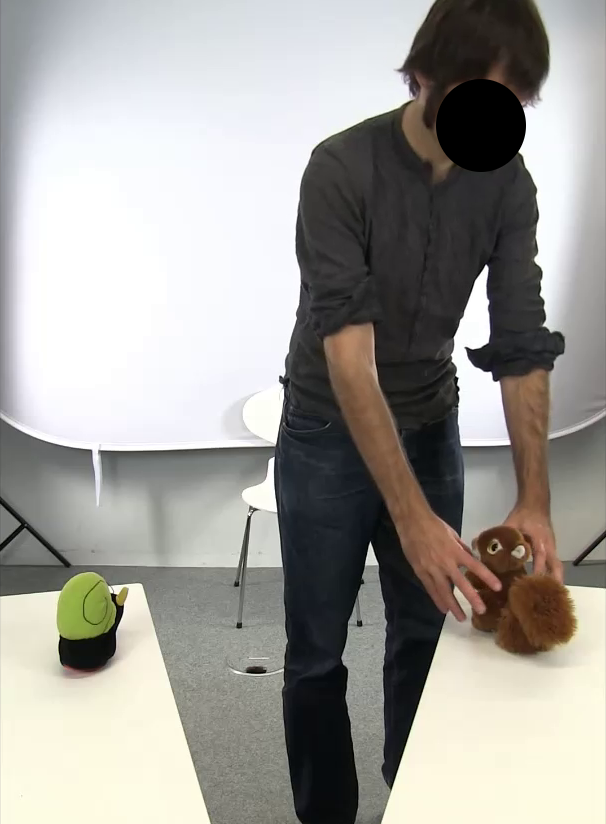
\includegraphics[height=5cm]{stimulus-human-toys-anon}
    }

    \subfigure[\emph{Sound} task, robot condition]{
        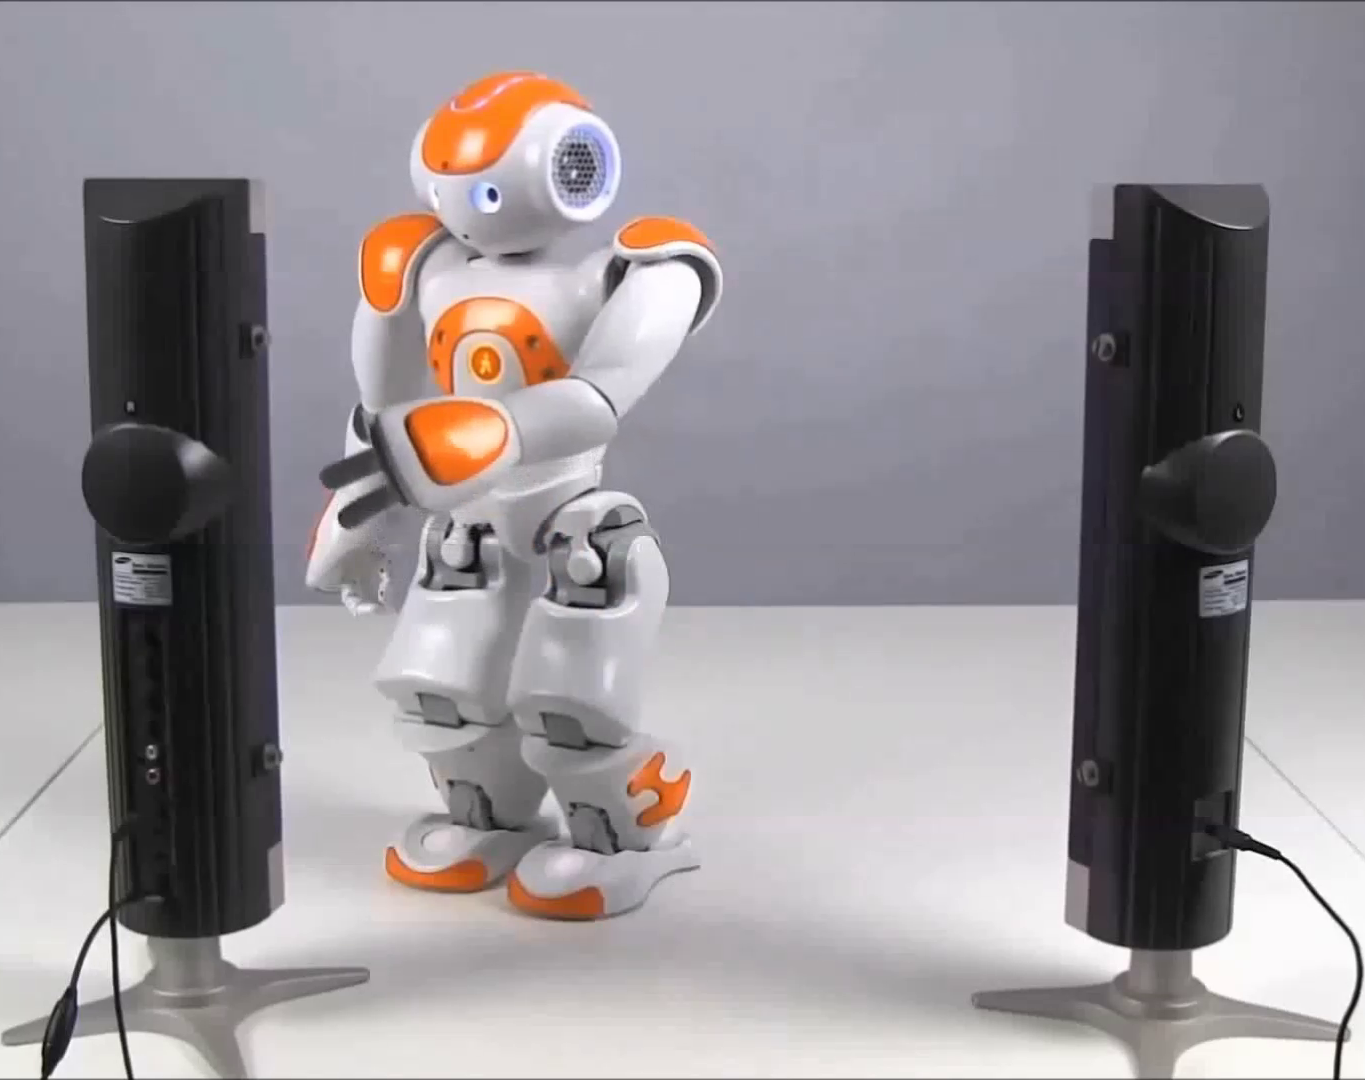
\includegraphics[height=5cm]{stimulus-robot-noise}
    }
    \subfigure[\emph{Sound} task, human condition]{
        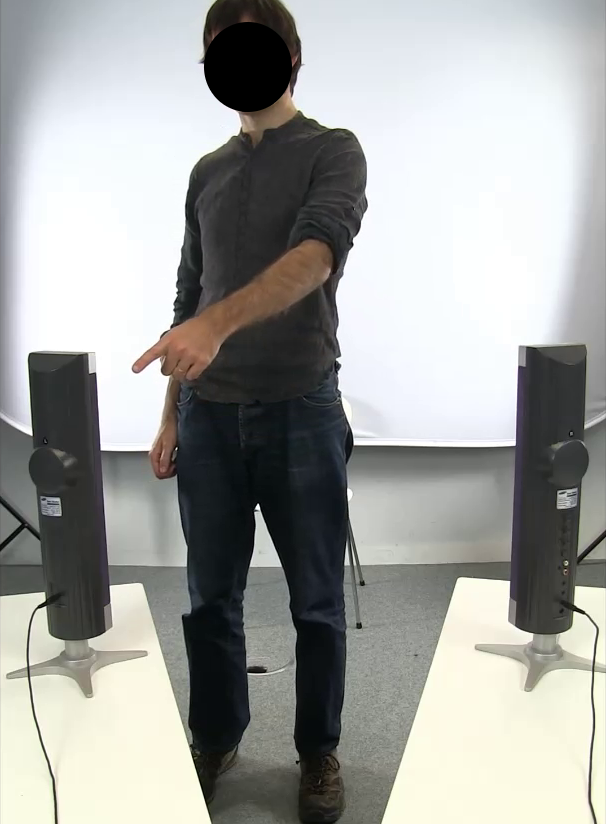
\includegraphics[height=5cm]{stimulus-human-noise-anon}
    }


    \caption{\small Screenshots of the 2$\times$2 stimuli. Note that the images above have been
    slightly cropped: the original video are framed so that the agent (robot or
    human) always remains entirely visible.}
    \label{fig:stimuli}
\end{figure}

Section~\ref{stimuli_design}, at the end of the article, specifically discusses
the design constraints that were accounted for while creating the above stimuli.

\subsection{Questionnaires}

Before starting the experiment, the participants were asked to fill a
pre-questionnaire which had 49 questions (5-point Likert scale). The
questionnaire comprised of questions assessing their familiarity with robots, 10
items from \emph{Big-Five} personality questionnaire, 15 questions taken from
Godspeed questionnaire (questions related to \emph{anthropomorphism},
\emph{likeability} and \emph{perceived intelligence}) and 20 questions rating
human-likeness (from~\cite{ruijten_introducing_2014})\footnote{The
the pre- and post-questionnaires are available online:
\url{https://github.com/chili-epfl/anthropomorphism-eyetracking}.}. The pre-questionnaire
typically took 5 minutes for participants to fill. The results were turned into
a score noted \anti (\emph{initial tendency to anthropomorphize}) following a
method presented below (section~\ref{questionnaires_processing}).

The post-questionnaire was administered at the end of the experiment, and was
close to the pre-questionnaire: the personality questions were omitted, and a
manipulation check question was added (\emph{``In your opinion, the tasks that
you watched were more: A robot kind of task ... A human kind of task''}).
This questionnaire typically took 3 to 4 minutes to fill. The resulting score is
noted \antf (\emph{final tendency to anthropomorphism}).

The difference \deltaant measured for each participant between the pre-
and post-questionnaires forms the dependent variable of our experiment. It
reflects the impact of the video stimuli on the anthropomorphic perception that
they have of robots \emph{in general}: the Godspeed questions used in the
questionnaires are not specific to the Nao robot used in this particular
experiment, and indeed assess how humans perceive robots in a broad sense.

\section{Experiment}

\subsection{Course of the study}

Figure~\ref{course_of_study} gives an overview of the protocol, detailed
hereafter.

\begin{figure}[ht!]
    \centering
    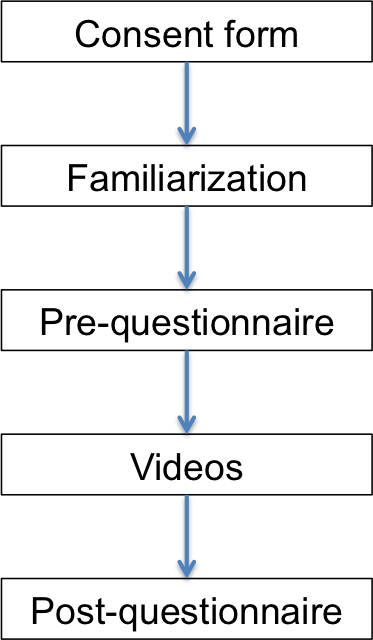
\includegraphics[width=0.3\linewidth]{experimentFlow}
    \caption{Overview of the course of the study}
    \label{course_of_study}
\end{figure}
\paragraph{Participants}

We ran first a pilot study with 10 participants, followed by an experiment with
56 subjects (mean age: 20.9, $SD=3.9$, 31 females and 25 males).
The participants were recruited amongst students of our university. To avoid
students with a high familiarity with robots and artificial intelligent systems,
Computer Science and Electronics curriculum were excluded. This was \textit{a
posteriori} comforted by the questionnaire responses: no participants
reported itself as being very familiar with robots, 8 reported some familiarity
and 7 out of 56 owned a domestic robot (vacuum cleaner).

The study lasted about 15 minutes per participant; each participant was invited
for one session only.

As stated previously, the study follows a 2$\times$2 design
(table~\ref{table:design}): the \emph{deep} \vs {shallow cognitive context}
condition was between-subject ( 30 subjects performed the \emph{deep cognitive}
tasks while 26 were in the \emph{shallow cognitive} condition); the \emph{robot}
\vs \emph{human} condition was within-subject (the order of stimuli presentation
was counter-balanced over the 56 participants).

\paragraph{Pre-questionnaire and familiarization}

Before the experiment, participants were made to read, understand and sign a
consent form. Participants were then asked to fill the 49 questions of
the pre-questionnaire, with a 10 minutes time limit that none of the participants
reached.

After the pre-questionnaire, we invited the participants to an initial
free interaction with a \textbf{powered-off} Nao robot (we did not constraint
the time, and participants played between 2 and 3 minutes with the robot).

The purpose of this pre-interaction was to get the participants acquainted with the
robot shape and kind of motions it could possibly perform, and therefore
mitigate the (visual) novelty effect (so that they do not get surprised seeing
a robot for the first time in the videos).

\paragraph{Videos}

After filling the pre-questionnaire, we conducted a brief eye-tracker
calibration procedure, and the participants' gaze was recorded while they
watched the \emph{robot} and \emph{human} interaction videos.

\paragraph{Post-questionnaire}

Finally, the participants were asked to fill the post-questionnaire.
Before leaving, each participant was given a reward
equivalent to EUR 10.

\subsection{Data Collection}

\subsubsection{Gaze variables}

\paragraph{Areas of interest}

As seen in figure~\ref{fig:aoi}, we defined 10 areas of interest (AOIs): one on
the head of the agent (robot or human), two on the arms (left and right), two on
the hands, two on the legs and one on the torso. Besides, we defined one area of
interest per toy or speaker (depending on the stimulus).

\begin{figure}
    \centering
    \subfigure[\emph{Picking} task, robot condition]
    {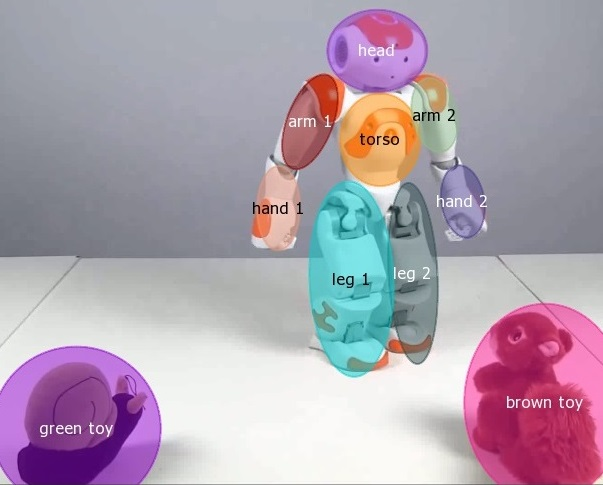
\includegraphics[height=5cm]{aoi-robot}\label{fig:aoi-toys}}
    \subfigure[\emph{Sound} task, human condition]
    {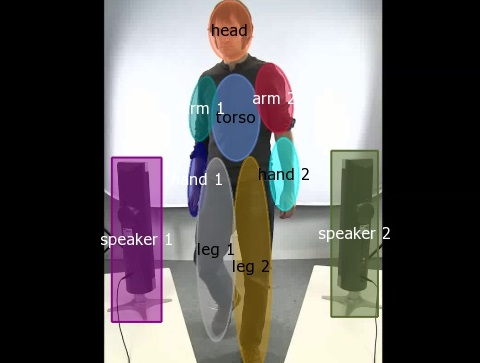
\includegraphics[height=5cm]{aoi-human}\label{fig:aoi-noise}}

    \caption{Areas of interest used for the gaze analysis}
    \label{fig:aoi}
\end{figure}

We recorded the fixations on one of these 10 zones and normalized by different total video duration and surface of AOIs between the robot and human conditions. We finally analyzed their distribution, producing what we
call \emph{gaze patterns}. The difference in the gaze patterns over ``N'' AOis can be calculated as follows:\\




\paragraph{Differences between gaze behaviours}

To compare gazing behaviours across conditions, we compute a \emph{difference in
gaze patterns} over the $N(=10)$ AOIs:

{\large
\[
    \delta_{\mathcal{H}, \mathcal{R}}^{\text{gaze}} =
    \frac{\sum\limits_{{\text{{\sc aoi}s}}}\left |
    \frac{\text{Time}_{\text{Human}}^{\text{\sc
aoi}}}{\text{Area}_{\text{Human}}^{\text{\sc aoi}}} -
\frac{\text{Time}_{\text{Robot}}^{\text{\sc
aoi}}}{\text{Area}_{\text{Robot}}^{\text{\sc aoi}}} \right |}{N}
\]
}

\emph{Time} and \emph{Area} are normalized, respectively for the total
video length and the total area of the AOIs.

\subsubsection{Questionnaires processing}
\label{questionnaires_processing}

Questionnaires were coded and two values, the \emph{initial tendency to
anthropomorphize} \anti and the \emph{final tendency to anthropomorphize} \antf
were computed, respectively from the pre- and post-questionnaires.

These values were computed by a direct sum of the rating provided by the
participants for the Godspeed's questions in the categories
\emph{anthropomorphism} and \emph{likeability}. These ten questions were rated
between -2 and 2, hence \anti and \antf vary between -20 and 20.  The other
questions (including the Big-Five personality test) were not used for this
study.

\section{Results}

Based on the experiments conducted on 55 participants in the human
($\mathcal{H}$) and robot ($\mathcal{R}$) interactions across \emph{shallow} and
\emph{deep cognitive context} conditions, we have the following
results.\footnote{The
detailed statistics and code used for obtaining the results are available here :
\url{https://github.com/chili-epfl/anthropomorphism-eyetracking}.}

\subsection{General Biases}

While testing for all the 4 hypotheses, we observed no significant bias with
respect to age, gender, EPFL status, familiarity with robot and robot ownership
of the participants, \ie there was no correlation found between these factors
and the gaze patterns in the videos.

\subsection{Manipulation check}

\begin{figure}
    \centering
    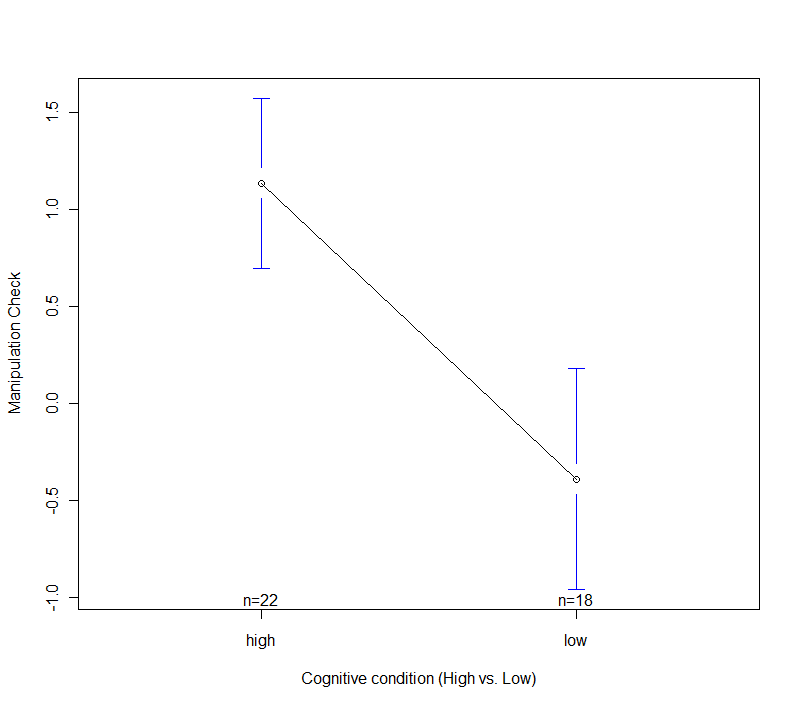
\includegraphics[width=7cm]{ManipulationCheck}
    \caption{Average ratings for the manipulation check question}
    \label{fig:ManipulationCheck}
\end{figure}


Participants were asked in the post-questionnaire whether the video presented a
\emph{``robot kind of task''} or a \emph{``human kind of task''} on a 5-points
scale (numerical values ranging from -2 to 2, where -2 refers to robot kind of
task). As can be seen in figure 2, we got a significant correlation in this
manipulation check ($F[1,54] = 29.0, p < .001$) which validates our manipulation
and supports \h{0}: the participants that were shown the \emph{shallow cognitive
context} videos identified the task as more robot-like and participants watching
\emph{deep cognitive context} videos perceived the tasks as more human-like. 


\subsection{Gaze differences between human and robot conditions}

We grouped the 8 areas of interest located on the agent into 4 categories : {\sf
head}, {\sf arms} (containing both arms and hands), {\sf torso}, {\sf legs}
(including both legs). Running an ANOVA against gaze fixations on the areas of
interest and the robot \vs human conditions, we obtain the following results:

{\sf head}: the fixations on the head for the human video
were observed to more than that for the robot video ($F[1,54] = 12.7, p < .001$)

{\sf arms}: the fixations on the arms for the $\mathcal{H}$ video
were also greater than that for the robot video ($F[1,54] = 16.5, p < .01$)

{\sf legs}: the fixations on the legs were much lower
for the human video as compared to the robot video ($F[1,54] = 1.9, p < .1$)

{\sf torso}: the fixations on the torso were higher for the
human video than for the robot video ($F[1,54] = 2.65, p < .1$) 

In summary, and over the duration of these shorts videos, the gaze behaviours
were significantly different between the robot and human conditions, supporting
\h{1}.

\subsection{Impact of the tendency to anthropomorphize on human
gazing behaviours}

We got a significant correlation between $\delta_{\mathcal{H},\mathcal{R}}$ and
the \anti. As can be seen in figure~\ref{h2}, there is a significant negative
correlation between the two quantities (Pearson Correlation Coefficient = -0.43,
$p < .001$).

\begin{figure}
    \centering
    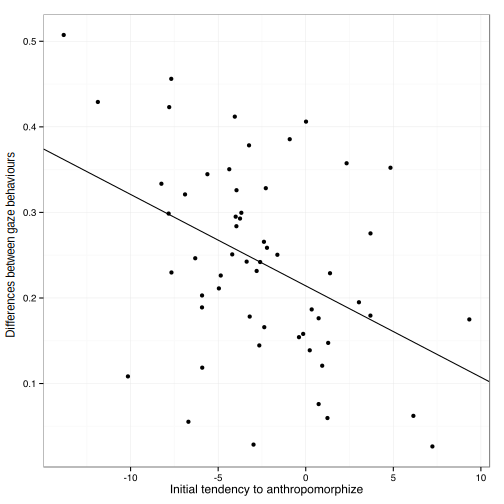
\includegraphics[width=3.3in]{H2}\label{GazeDifference-vs-ICA}
    \caption{Difference in gaze patterns $\delta_{\mathcal{H},
    \mathcal{R}}^{\text{gaze}}$ \vs \anti}
    \label{h2}
\end{figure}

\subsection{Gaze behaviours in shallow \vs deep cognitive contexts}

We analysed these possible correlations for robot condition only: the human case is
inherently a source of deep cognitive context, hiding the effects of our
manipulation on a shallow \vs deep cognitive context.

Based on ANOVA results, taking the 5 groups of AOIs {\sf head}, {\sf arms}, {\sf
hands}, {\sf torso}, {\sf legs} for the robot in both the shallow and deep
cognitive context conditions, the fixations on the head in the deep condition
were found to be significantly higher than that in the shallow condition
($F[1,54] = 4.2, p < .05$). For all other AOIs groups, the fixations across
shallow and deep conditions were almost the same. Figure~\ref{h3} shows the
distribution of proportion of time spent gazing on the 5 AOIs for the two
conditions.

\begin{figure}
    \centering
    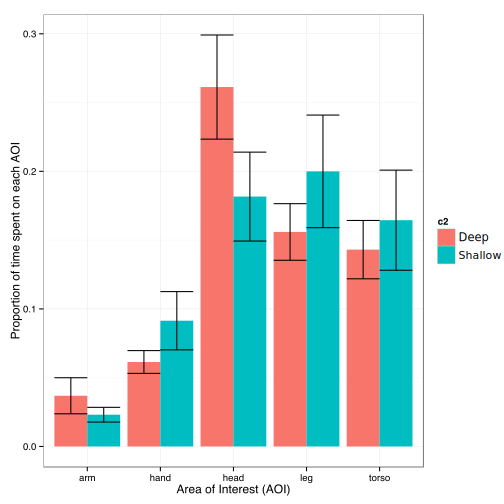
\includegraphics[width=3.3in]{GazeHighLow}\label{GazeHighLow}
    \caption{Gaze fixations on the different areas on interest, for shallow \vs
    deep cognitive context conditions.}
    \label{h3}
\end{figure}

This constitutes the main result of this study: inducing a deeper cognitive
context for the same interaction suffices to lead to significantly longer
fixations on the agent's head.

\subsection{Correlation between cognitive context and changes in anthropomorphic
attributions}

Running an ANOVA against the evolution of anthropomorphic attributions
(\deltaant) over the duration of the experiment, in the two cognitive
conditions, shows that \deltaant is greater for tasks with a deeper cognitive
context than that for the shallow cognitive tasks ($F[1,54] = 6.54, p < .05$,
figure~\ref{h4}). In other words, after being exposed to short videos of a robot
performing simple tasks, subjects primed with a deeper cognitive context report
a significantly higher tendency to anthropomorphize robots \emph{in general} (as
the questionnaires on anthropomorphic attributions explicitely refered to
\emph{robots in general}).

\begin{figure}
    \centering
    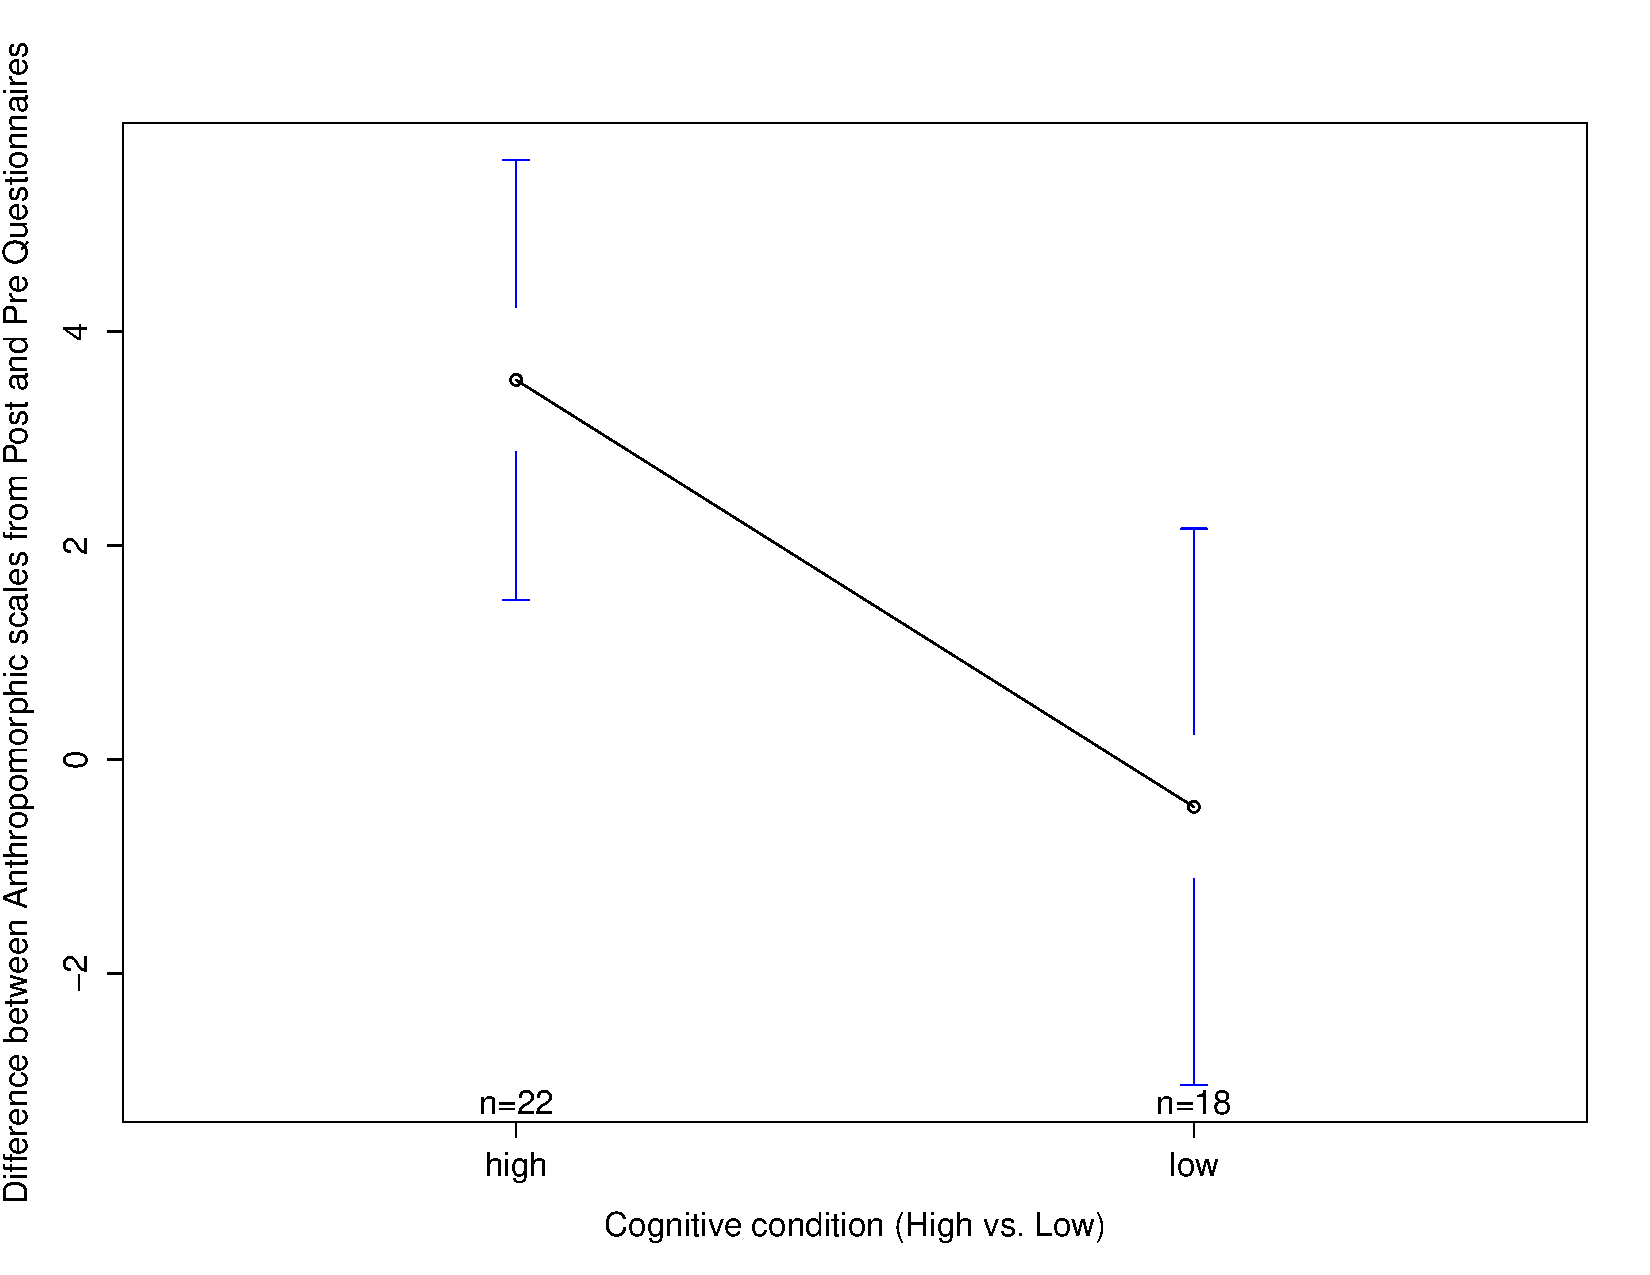
\includegraphics[width=3.3in]{H4}\label{ICAtoAAPImprovement}
    \caption{Difference between \anti and \antf in the shallow and deep
    cognitive contexts.}
    \label{h4}
\end{figure}

This result supports \h{4} and validate that the cognitive context impacts the
attribution of anthropomorphic features to robots. This, in turn, supports the
\emph{proxy} hypothesis of \h{3}: \emph{head fixations are a proxy for higher
levels of human-likeness attributions}.

%%%%%%%%%%%%%%%%%%%%%%

\section{Discussion and Conclusion}

\subsection{Discussion of the results}

The presented results bring some light on our initial hypotheses.

The clearly significant correlation between deep \vs shallow conditions and the
answers to the question \emph{Were the task more robot-like or human-like?}
proves that our manipulation was successful, and that a shallow cognitive
context was indeed associated to a robot-like situation, while a deeper
cognitive context was associated to a human-like situation (\h{0}).

The hypothesis \h{1} postulated that the gaze behaviours alone could tell if the
subjects was observing a robot or a human. Indeed, our results show
significantly different (normalized) fixations: the gaze distribution of a human
observer are different for humans and robots.

Hypothesis \h{2} looked at a possible interaction between our potential to
anthropomorphize (as measured in the pre-questionnaire) and our actual gaze
behaviour, the hypothesis being that high anthropomorphizers would show smaller
differences between the way they look at robots and humans (since they would
consider robots closer to humans than low anthropomorphizers). Our data supports
this hypothesis: participants reporting an higher tendency to anthropomorphize
tend to have similar gazing behaviours whether they look at humans or at robots.

To rephrase it: statistically speaking, your tendency to anthropomorphize things
is reflected in the way you look at these things: you will also look at them
\emph{as if they were humans}.

The third hypothesis \h{3} proposes that head fixations are related to the
cognitive context, which is clearly supported by our data: in deeper cognitive
context, one tends to spend more time looking at the head of the interacting
agent than in a shallow cognitive context. We also hypothesized that, in turn,
head fixations could act as a \emph{proxy to anthropomorphic projections}: as
underlined in the previous section, our data also support this second
hypothesis.

Finally, the hypothesis \h{4} looks at the dynamic of anthropomorphic
projections, with the hypothesis that watching an interaction with a particular
robot in a deeper cognitive context may impact \emph{globally} the
anthropomorphic perceptions of robots. This is supported by our study.

\subsection{Summary and Contributions}

The study and results presented in this article lead to two main contributions:
new insights on the impact of the cognitive context of the interaction on the
perception of a robot by humans; a novel unbiased methodology based on
eye-tracking to measure anthropomorphic attributions during a running
human-robot interaction.

Our first contribution extends our understanding of the attribution of
human-like characteristics to robot by exploring the role of the interaction
context. As we show in the article, it appears that \textbf{even relatively
subtle context priming may lead to significantly different anthropomorphic
perceptions of the exact same robot, performing the exact same task}, as
confirmed both by distinct gaze patterns, and different reported perceptions in
questionnaires. To the best of our knowledge, this effect had not been previously
evidenced.

This leads to a second-order effect that we also evidence here: depending on the
cognitive context, the tendency to attribute human-like characteristics to robot
\textbf{evolves} in significantly different ways: after observing a robot in a
context that pre-suppose deeper cognitive capabilities, \textbf{people increase
their general tendency to anthropomorphize robots} compared to a shallow
cognitive context, even though the robot appearance and visual behaviour is the
exact same.

The second contribution is a methodological one: we present in this article
\textbf{a novel technique to assess anthropomorphic projections that relies on a
biometric measurement (eye-tracking) to compare gaze fixation durations on
the face of the robot}. We cross-validate this new metric with existing,
established, questionnaires. Compared to current techniques (post-hoc
annotations of videos and questionnaires), this new approach is objective,
is less impacted by experimental biases (like the \emph{observer effect},
where the subject's behaviour is impacted by the fact he/she knows that
he/she is observed) and take place during the interaction itself
(\emph{in-the-moment} measurement).

Besides, we also introduce a new kind of visual stimuli, specifically designed
to study the impact of non-appearance, non-behavioural related effects on the
human-like perception of robots. We make these video stimuli available to the
community, and therefore invite our colleagues to reproduce our experimental
results. The next section describe the specificities of these stimuli, and also
discuss how such a methodology can apply to real-world scenarios.

As a whole, the article attempts to contribute to our understanding of an
intricate psychological effects that come to play when humans and robots
interact, both in terms of methodology and experimental evidence.

\subsection{Design of the stimuli and applicability of the method to real world
scenarios}
\label{stimuli_design}

The video stimuli had to obey to several constraints: they had to depict
plausible and legible situations, yet simple enough to be suitable for an
eye-tracking study (simple mechanics, easily distinguishable elements at
predictable locations). The body parts of the robot or human would need remain
visible most of the time. The actions had to be meaningful for both a robot and
a human, and both should be able to perform them in similar ways (similar pace,
similar movements) without looking ackward.

Finally, the situations needed to support two possible cognitive contexts
(shallow \vs deeper cognitive context), and triggering one or the other of these
contexts needed to be done \emph{without changing} the visual part of the
stimulus.

We initially prepared three different stimuli: the \emph{Picking} task, the
\emph{Sound} task and a \emph{Dance} task.  During the \emph{Dance} task, the
agent was either asked to \emph{``Show some movements''} (\emph{shallow
cognitive context} condition) or to \emph{``Dance with the music''}
(\emph{deeper cognitive context} condition). While all the participants were
shown this stimuli as well, we decided to exclude it from the results as the
nature of the task (participants had to watch body movements) defeated our
gaze-based investigation method: the subjects expectedly paid attention to the
whole body of the robot or human (even distribution of the gazes on the body),
thus making specific gaze patterns on the head difficult to evidence.

This underlines the difficulty of designing appropriate stimuli and raises the
question of the applicability of our method to real-world, ``in the wild''
human-robot interaction.

Two main comments can be made: first, we had to carefully design those stimuli
to \emph{evidence} the link between the (anthropomorphic) perception of a robot
and actual gaze fixations on the face of the robot. This being granted,
researchers will not have to design their scenarios in such a constraint way to
rely on our result, \ie the link between perception and gaze behaviour.

Besides, one may point that, in real-world experiments, the robot does not
always remain in the field of view of the subject, and, at the very least, the
body of the robot may be partially occluded at time.  This is certainly true,
and while new experiments would be welcome to validate it, we believe that our
method remains effective in these situations. First it relies on the
\emph{ratio} of the gaze fixations on the head \vs gaze fixations on other parts
of the body, thus compensating for out-of-sight robots; second, our method
\emph{does not} provide an \emph{absolute} measurement of the level
anthropomorphic perception, but rather a \emph{relative} measurement: within a
group of subject, it enables to classify subjects in term of their level of
projected anthropomorphism onto the robot.  This means that, while this method
can not be used to assess the perception of robots between different interaction
situations (\ie different experiments), it can be employed within a group a
subjects taking part to the same experiment.

Lastly, the stationary eye-tracker would also have to be replaced by a mobile
eye-tracker. This would however not impact the interpretation of the results.

%\subsection{Context and Interaction Design}
%
%\fxwarning{discuss here how context can be used to shape the interaction}
%
%
%Anthropomorphism as a proxy for cognitive/affective bonds that are esthablishing
%between humans and robots.
%
%\fxnote{discuss extensions towards mobile eyetrackers}
%
\bibliographystyle{apacite}
\bibliography{biblio}

%\appendix
%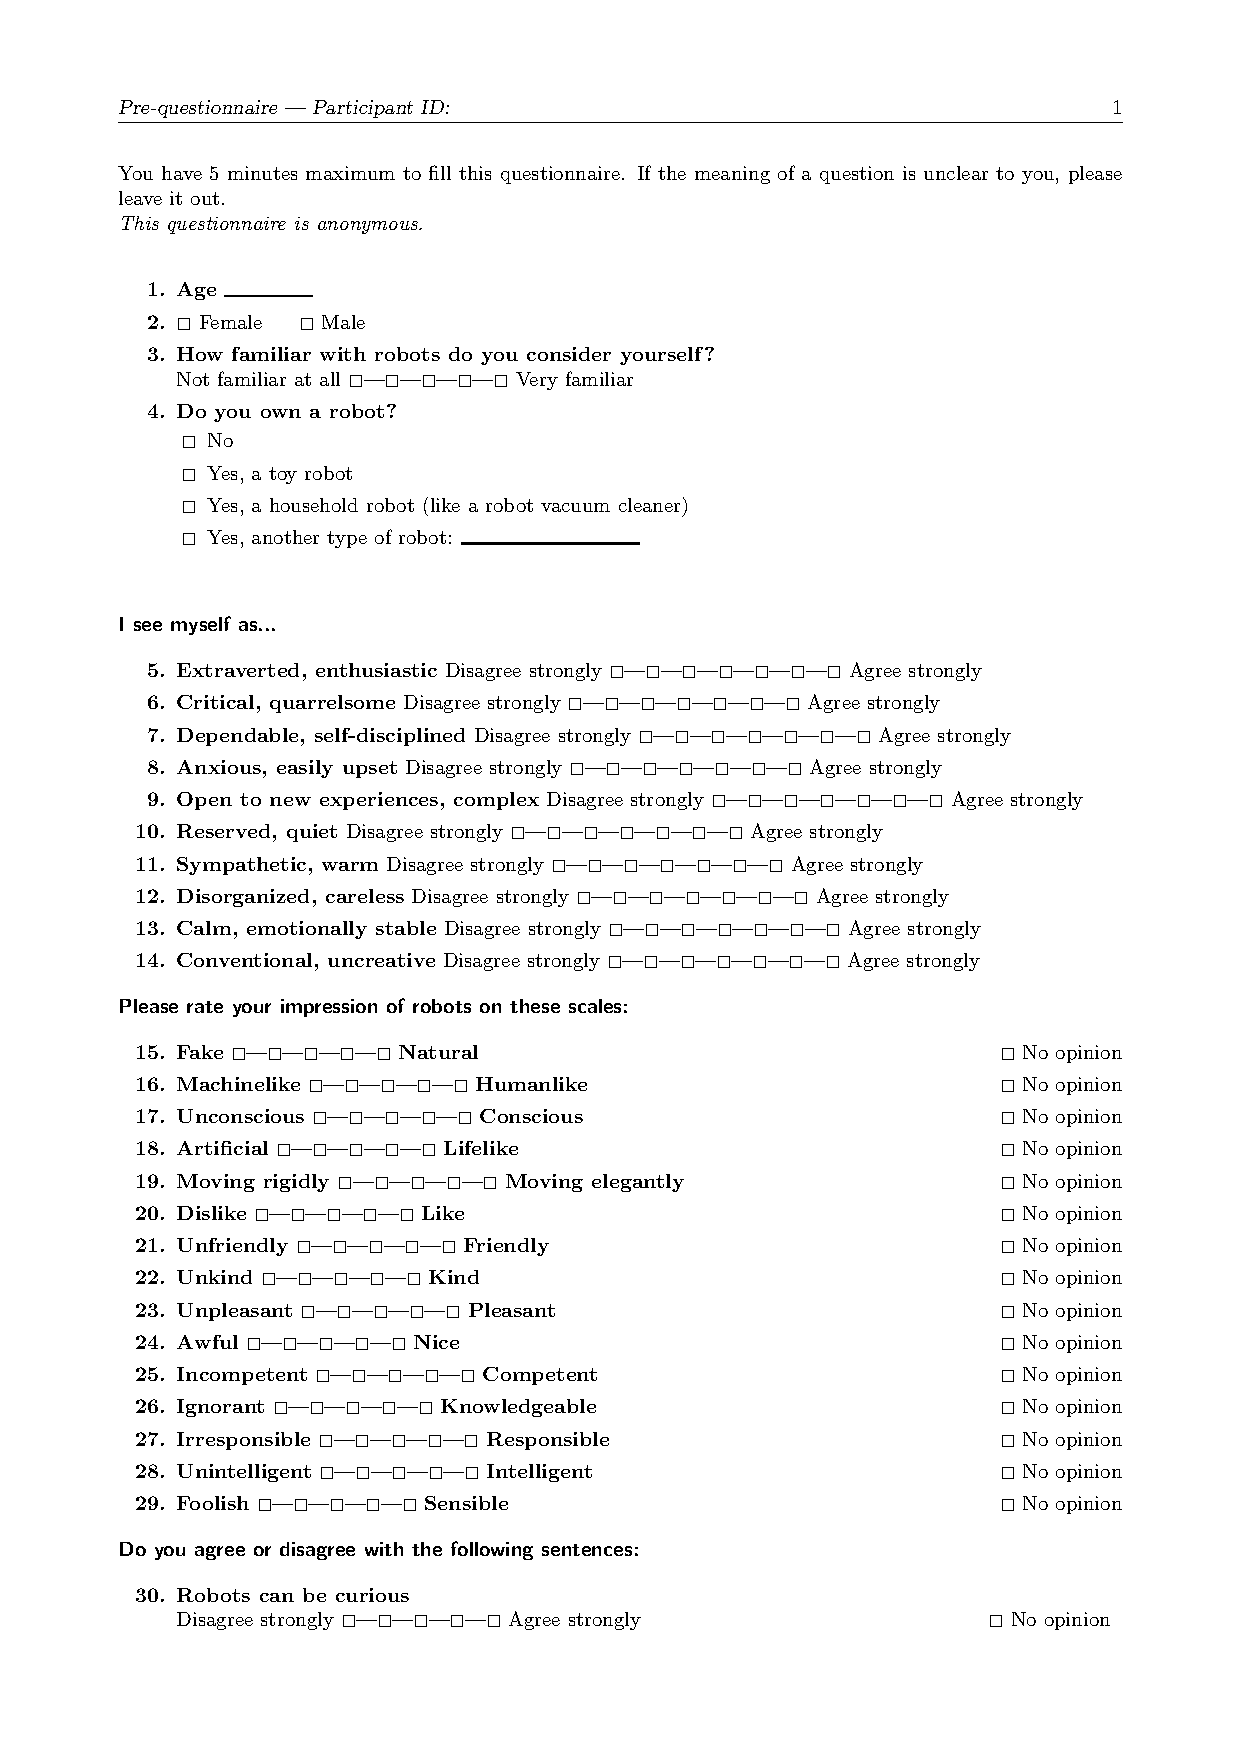
\includepdf[pages={1,2}]{pre-questionnaire.pdf}
%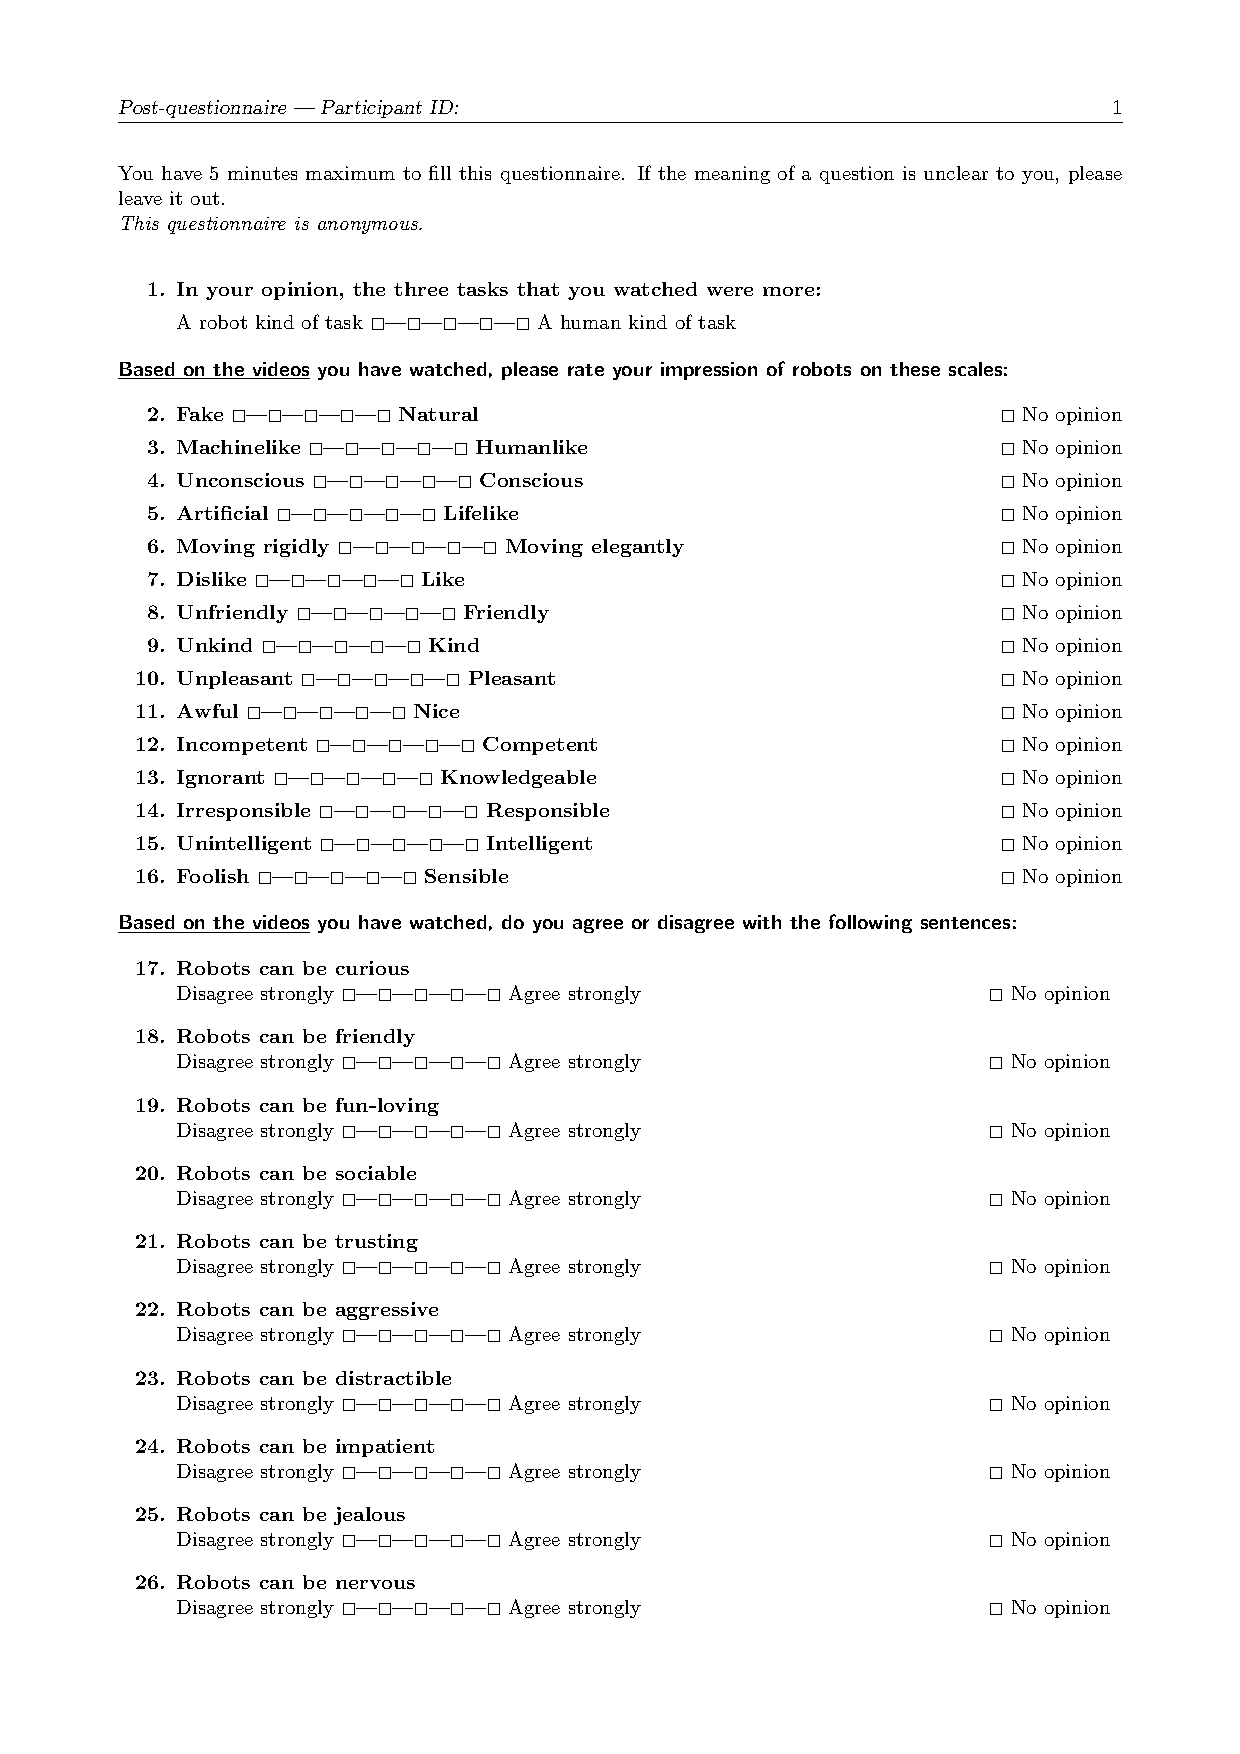
\includepdf[pages={1,2}]{post-questionnaire.pdf}

\end{document}
